\documentclass[a4paper,14pt]{article}
\usepackage{float}
\usepackage{extsizes}
\usepackage{amsmath}
\usepackage{amssymb}
\everymath{\displaystyle}
\usepackage{geometry}
\usepackage{fancyhdr}
\usepackage{multicol}
\usepackage{graphicx}
\usepackage[brazil]{babel}
\usepackage[shortlabels]{enumitem}
\usepackage{cancel}
\usepackage{textcomp}
\usepackage{array}
\usepackage{longtable}
\usepackage{booktabs}
\usepackage{float}   % Para usar o modificador [H]

\columnsep=2cm
\hoffset=0cm
\textwidth=8cm
\setlength{\columnseprule}{.1pt}
\setlength{\columnsep}{2cm}
\renewcommand{\headrulewidth}{0pt}
\geometry{top=1in, bottom=1in, left=0.7in, right=0.5in}

\pagestyle{fancy}
\fancyhf{}
\fancyfoot[C]{\thepage}

\begin{document}
	
	\noindent\textbf{6FMA31 - Matemática} 
	
	\begin{center}Sentenças, equações, inequações e conjunto verdade (Versão estudante)
	\end{center}
	
	\noindent\textbf{Nome:} \underline{\hspace{10cm}}
	\noindent\textbf{Data:} \underline{\hspace{4cm}}
	
	%\section*{Questões de Matemática}
	
	~ \\
	\noindent\textbf{Sentença declarativa} é toda expressão à qual podemos dar o valor de verdadeiro ou falso. Para simplificar, usamos apenas a expressão sentença. \\
	Expressões do tipo $x = 2$, por exemplo, são chamadas \textbf{sentenças abertas}, pois tal afirmação não é verdadeira nem falsa. Se substituirmos $x$ por 2, teremos 2 = 2, o que é verdadeiro; por outro lado, se substituirmos $x$ por 3, obteremos 3 = 2, o que é falso. \\
	Sentença e sentença aberta também recebem o nome \textbf{forma sentencial}. \\\\
	As letras que aparecem em uma sentença aberta são chamadas \textbf{variáveis} (ou \textbf{incógnitas}).
	Sentenças do tipo $F = G$ são chamadas \textbf{equações}. Se no lugar de "=" aparece o sinal ">" ou "$\geq$" ou "<" ou "$\leq$", temos uma \textbf{inequação}. \\
	O conjunto que escolhemos para substituir a letra em uma sentença aberta chama-se \textbf{conjunto universo}. \\
	Os valores do conjunto universo que tornam a sentença verdadeira formam o \textbf{conjunto verdade}. \\
	\noindent\textsubscript{~-----------------------------------------------------------------------------------------------------------------------------------------------------------}
    \begin{multicols}{2}
    	\begin{enumerate}
    		\item Escreva quais das expressões abaixo são sentenças.
    		\begin{enumerate}[a)]
    			\item Eu gosto de nadar. \\\\
    			\item Não é verdade que seis é maior que dez. \\\\
    			\item Todos os homens usam gravatas. \\\\
    			\item A sua casa é a da esquina? \\\\
    			\item Três mais dois. \\\\
    			\item Dois. \\\\
    			\item 5 + 1 = 6 \\\\
    			\item 5 + 0 = 0 \\\\
    			\item 10 é maior. \\\\
    			\item Bem-vindo. \\\\
    			\item 8 é maior que 4. \\\\
    			\item 6 é múltiplo de 3. \\\\
    			\item \textit{A hora da estrela} foi escrito por Clarice Lispector. \\\\
    		\end{enumerate}
    		\item Escreva 5 sentenças envolvendo números. Substitua a ocorrência de um nome ou a descrição de número por uma letra, em cada sentença, para obter sentenças abertas.
    		
    		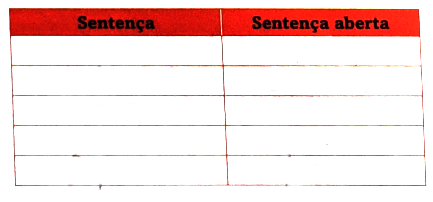
\includegraphics[width=1\linewidth]{imagens_6MFA31/tabela1}
    		\item Em cada item é dada uma sentença aberta e um conjunto universo para ela. Apresentar o conjunto verdade.
    		\begin{enumerate}[a)]
    			\item $x - 1 = 4, U = \{1, 3, 5\}$ \\\\
    			\item $y < 8, U = \{-1, 5, 10, 15\}$ \\\\
    			\item $x = x, U = \{2, 4, 6, 8, 10\}$ \\\\
    			\item $y = y + 3, U = \{2, 3, 4, 5\}$ \\\\
    			\item $a = a, U = \mathbb{Z}$ \\\\
    			\item $x = x -2, U = \mathbb{Z}$ \\\\
    			\item $j = 4, U = \mathbb{Z}$ \\\\
    			\item $z \leq 2, U = \{-2, 0, 2, 3\}$ \\\\
    		\end{enumerate}
    		\item Escreva quais das expressões abaixo são sentenças declarativas.
    		\begin{enumerate}[a)]
    			\item 6 + 4 = 10 \\\\\\\\
    			\item 6 + 3 = 9 \\\\\\\\
    			\item Não é verdade que misturar azul com amarelo resulta em verde. \\\\\\\\
    			\item Bom dia. \\\\\\\\
    			\item Dez. \\\\\\\\
    			\item Você aceita chá? \\\\\\\\
    			\item A Terra é redonda. \\\\\\\\
    			\item Seja bem-vindo! \\\\\\\\
    		\end{enumerate}
    	    \item Escreva três sentenças envolvendo números. Substitua a ocorrência de um nome ou descrição de número por uma letra, em cada sentença, para obter sentenças abertas.
    	    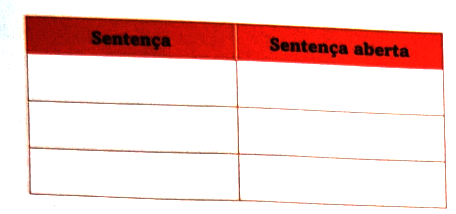
\includegraphics[width=1\linewidth]{imagens_6MFA31/tabela2}
    	    \item Em cada item é dada uma sentença aberta e um conjunto universo para ela. Apresente o conjunto verdade.
    	    \begin{enumerate}[a)]
    	    	\item $x - 2 = x \\ U = \{-2, -1, 0, 1, 2\}$ \\\\
    	    	\item $x = x ~~~~~~ U = \mathbb{Z}$ \\\\\\\\
    	    	\item $\frac{x}{x} = 1 ~~~~~~ U = \mathbb{Z_+}$ \\\\
    	    	\item $y$ é ímpar ~~~~~~ $U = \mathbb{Z}$ \\\\
    	    	\item $\alpha > 2 ~~~~~~ U = \{0, 1, 2, 3, 4\}$ \\\\
    	    	\item $u = 1 ~~~~~~ U = \mathbb{Z}$ \\\\\\\\
    	    	\item $x = \frac{1}{x} ~~~~~~ U = \{1, 3, 5\}$ \\\\
    	    \end{enumerate}
            \item Escreva duas equações e três inequações. Escolha em cada uma delas um conjunto universo e apresente o conjunto verdade.
            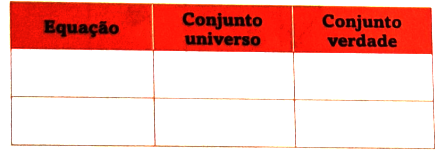
\includegraphics[width=1\linewidth]{imagens_6MFA31/tabela3}
            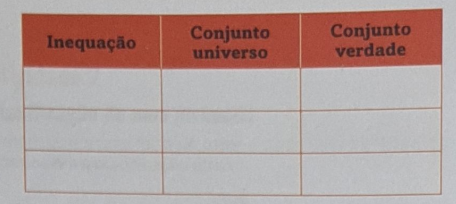
\includegraphics[width=1\linewidth]{imagens_6MFA31/tabela4}
    	\end{enumerate}
    \end{multicols}
\end{document}